\subsection{Subgraphs of the Comparability Grid}

Recall that, by Fact \ref{fact:vertex-deletion}, vertex deletion is an operation allowable in the Measurement Calculus model of MBQC. Thus, if we can show that a family of induced subgraphs of comparability grids is universal, we obtain that comparability grids are universal. We begin by characterizing the data of a subgraph of a comparability grid.

\begin{fact}
\label{fact:tuple-construction}
Let \(H\) be an induced subgraph of a comparability grid \(\CGrid\), with
\(|V(H)|=n\). Then \(H\) admits a canonical encoding by a permutation
\(\pi(H)\in S_n\). Conversely, every permutation \(\pi\in S_n\) determines
an induced subgraph \(H(\pi)\) of \(\CGrid\).
\end{fact}

\begin{proof}
Write the vertices of \(H\) as points \((x,y)\) in the comparability grid,
where two vertices are adjacent precisely when they are comparable:
\begin{align}
    (x_1,y_1)(x_2,y_2)\in E(H)
    &\iff (x_1-x_2)(y_1-y_2)>0.
\end{align}
Define a perturbed point set
\begin{align}
    V'
    &:= \left\{
        \left(x+\frac{y}{n+1},\ y+\frac{x}{n+1}\right)
        : (x,y)\in V(H)
    \right\}.
\end{align}
\begin{figure}[H]
\centering
\begin{tikzpicture}[
    scale=1.3,
    dot/.style={circle, inner sep=1.5pt},
    faintdot/.style={dot, fill=black!25},
    sel/.style={dot, fill=black},
    faintedge/.style={line width=0.55pt, draw=black!25},
    seledge/.style={line width=0.85pt, draw=black},
    lab/.style={draw=none, fill=none, inner sep=0pt, font=\small},
]

\begin{scope}[xshift=0cm]
    % vertices
    \foreach \x in {1,2,3}{
    \foreach \y in {1,2,3}{
        \node[faintdot] (L-\x-\y) at (\x,\y) {};
    }
    }

    % select vertices (2,1), (1,2), (2,3), (3,2)
    \node[sel] (Lsel-2-1) at (2,1) {};
    \node[sel] (Lsel-1-2) at (1,2) {};
    \node[sel] (Lsel-2-3) at (2,3) {};
    \node[sel] (Lsel-3-2) at (3,2) {};

    % (faint) edges of CGrid_{3x3} copied from your reference
    \draw[faintedge] (L-1-1) -- (L-1-2);
    \draw[faintedge] (L-1-1) -- (L-2-1);
    \draw[faintedge] (L-1-1) -- (L-2-2);
    \draw[faintedge] (L-1-1) -- (L-2-3);
    \draw[faintedge] (L-1-1) -- (L-3-2);

    \draw[faintedge] (L-1-2) -- (L-1-3);
    \draw[faintedge] (L-1-2) -- (L-2-2);
    \draw[faintedge] (L-1-2) -- (L-2-3);

    \draw[faintedge] (L-1-3) -- (L-2-3);

    \draw[faintedge] (L-2-1) -- (L-2-2);
    \draw[faintedge] (L-2-1) -- (L-3-1);
    \draw[faintedge] (L-2-1) -- (L-3-2);

    \draw[faintedge] (L-2-2) -- (L-2-3);
    \draw[faintedge] (L-2-2) -- (L-3-2);

    \draw[faintedge] (L-2-3) -- (L-3-3);
    \draw[faintedge] (L-3-1) -- (L-3-2);
    \draw[faintedge] (L-3-2) -- (L-3-3);

    \draw[faintedge] (L-1-1) to[bend left=20] (L-1-3);
    \draw[faintedge] (L-2-1) to[bend left=20] (L-2-3);
    \draw[faintedge] (L-3-1) to[bend left=20] (L-3-3);

    \draw[faintedge] (L-1-1) to[bend right=20] (L-3-1);
    \draw[faintedge] (L-1-2) to[bend right=20] (L-3-2);

    \draw[faintedge] (L-1-1) to[bend right=20] (L-3-3);
    \draw[faintedge] (L-1-2) -- (L-3-3);
    \draw[faintedge] (L-1-3) to[bend right=20] (L-3-3);

    \draw[faintedge] (L-2-1) -- (L-3-3);
    \draw[faintedge] (L-2-2) -- (L-3-3);

    % chosen subgraph edges among the 4 chosen vertices
    \draw[seledge] (L-2-1) -- (L-3-2);
    \draw[seledge] (L-2-1) -- (L-2-3);
    \draw[seledge] (L-1-2) -- (L-3-2); 
    \draw[seledge] (L-1-2) -- (L-2-3);

    % corner labels (optional)
    \node[lab, anchor=east] at ($(L-1-1)+(-0.25,0)$) {$(1,1)$};
    \node[lab, anchor=east] at ($(L-1-3)+(-0.25,0)$) {$(1,3)$};
    \node[lab, anchor=west] at ($(L-3-1)+(0.25,0)$) {$(3,1)$};
    \node[lab, anchor=west] at ($(L-3-3)+(0.25,0)$) {$(3,3)$};
\end{scope}

% ---------------------------
% Arrow to sheared grid
% ---------------------------
\draw[->,thick] (3.5,2) to (6.5,2);

% ---------------------------
% Helper: middle grid (shear/shift y by 0.2*(x-1))
% (x,y) -> (x, y + 0.2*(x-1))
% ---------------------------
\begin{scope}[xshift=6cm]
    % vertices
    \foreach \x in {1,2,3}{
    \foreach \y in {1,2,3}{
        \pgfmathsetmacro{\dx}{0.2*(\y-1)} % shift x depending on y
        \pgfmathsetmacro{\dy}{0.2*(\x-1)} % shift y depending on x
        \node[faintdot] (M-\x-\y) at (\x+\dx,\y+\dy) {};
    }
    }

    % select vertices
    \node[sel] (Msel-2-1) at (2,1+0.2) {};
    \node[sel] (Msel-1-2) at (1+0.2,2) {};
    \node[sel] (Msel-2-3) at (2+0.4,3+0.2) {};
    \node[sel] (Msel-3-2) at (3+0.2,2+0.4) {};

    % faint edges: same adjacency, just using shifted coordinates
    \draw[faintedge] (M-1-1) -- (M-1-2);
    \draw[faintedge] (M-1-1) -- (M-2-1);
    \draw[faintedge] (M-1-1) -- (M-2-2);
    \draw[faintedge] (M-1-1) -- (M-2-3);
    \draw[faintedge] (M-1-1) -- (M-3-2);

    \draw[faintedge] (M-1-2) -- (M-1-3);
    \draw[faintedge] (M-1-2) -- (M-2-2);
    \draw[faintedge] (M-1-2) -- (M-2-3);

    \draw[faintedge] (M-1-3) -- (M-2-3);

    \draw[faintedge] (M-2-1) -- (M-2-2);
    \draw[faintedge] (M-2-1) -- (M-3-1);
    \draw[faintedge] (M-2-1) -- (M-3-2);

    \draw[faintedge] (M-2-2) -- (M-2-3);
    \draw[faintedge] (M-2-2) -- (M-3-2);

    \draw[faintedge] (M-2-3) -- (M-3-3);
    \draw[faintedge] (M-3-1) -- (M-3-2);
    \draw[faintedge] (M-3-2) -- (M-3-3);

    \draw[faintedge] (M-1-1) to[bend left=20] (M-1-3);
    \draw[faintedge] (M-2-1) to[bend left=20] (M-2-3);
    \draw[faintedge] (M-3-1) to[bend left=20] (M-3-3);

    \draw[faintedge] (M-1-1) to[bend right=20] (M-3-1);
    \draw[faintedge] (M-1-2) to[bend right=20] (M-3-2);

    \draw[faintedge] (M-1-1) to[bend right=20] (M-3-3);
    \draw[faintedge] (M-1-2) -- (M-3-3);
    \draw[faintedge] (M-1-3) to[bend right=20] (M-3-3);

    \draw[faintedge] (M-2-1) -- (M-3-3);
    \draw[faintedge] (M-2-2) -- (M-3-3);

    % chosen subgraph edges (same adjacency)
    \draw[seledge] (M-2-1) -- (M-3-2);
    \draw[seledge] (M-2-1) -- (M-2-3);
    \draw[seledge] (M-1-2) -- (M-3-2); 
    \draw[seledge] (M-1-2) -- (M-2-3);

    % corner labels (optional, now reflecting shear)
    \node[lab, anchor=east] at ($(M-1-1)+(-0.25,0)$) {$(1.2,1.2)$};
    \node[lab, anchor=east] at ($(M-1-3)+(-0.25,0)$) {$(1.6,3.2)$};
    \node[lab, anchor=west] at ($(M-3-1)+(0.25,0)$) {$(3.2,1.6)$};
    \node[lab, anchor=west] at ($(M-3-3)+(0.25,0)$) {$(3.6,3.6)$};
\end{scope}
\end{tikzpicture}
\caption{The pertubation of $H(2143)$ in a $\CGrid_{3\times3}$.}
\label{fig:pertubed-cgrid}
\end{figure}
This perturbation preserves the relative comparability of every pair of
vertices, but ensures that no two vertices have the same first coordinate and
no two vertices have the same second coordinate. Indeed, if
\begin{align}
    x_1+\frac{y_1}{n+1}
    = x_2+\frac{y_2}{n+1}
    \Rightarrow
    x_1-x_2
    = \frac{y_2-y_1}{n+1}.
\end{align}
The left-hand side is an integer, while the right-hand side has absolute value
strictly less than \(1\). Hence both sides are \(0\), so \(x_1=x_2\) and
\(y_1=y_2\). Thus the vertices are identical. The same argument applies to the
second coordinates.

Now sort the perturbed vertices by increasing first coordinate. Since the
second coordinates are all distinct, their relative order is a permutation of
\([n]\). Denote this permutation by \(\pi(H)\). Thus, after relabeling the
vertices by their \(x\)-order, we may write the vertices as
\begin{align}
    v_i=(i,\pi(H)(i)), \qquad i\in[n].
\end{align}
The adjacency rule becomes
\begin{align}
    v_i v_j \in E(H)
    &\iff (i-j)\bigl(\pi(H)(i)-\pi(H)(j)\bigr)>0.
\end{align}
Hence \(H\) is exactly the permutation graph encoded by \(\pi(H)\).

Conversely, given \(\pi\in S_n\), define
\begin{align}
    V(H(\pi)) := \{(i,\pi(i)) : i\in[n]\},
\end{align}
with the induced comparability grid edges. This gives an induced subgraph
\(H(\pi)\subseteq \CGrid\).
\end{proof}

\begin{fact}
\label{fact:tuple-not-unique}
Two induced subgraphs \(H,H'\) of a comparability grid may satisfy
\(\pi(H)\neq \pi(H')\) while still being isomorphic as abstract graphs.
\end{fact}

\begin{proof}
Consider the permutations
\begin{align}
    \pi = 132,
    \qquad
    \sigma = 213.
\end{align}
\begin{figure}[H]
\centering
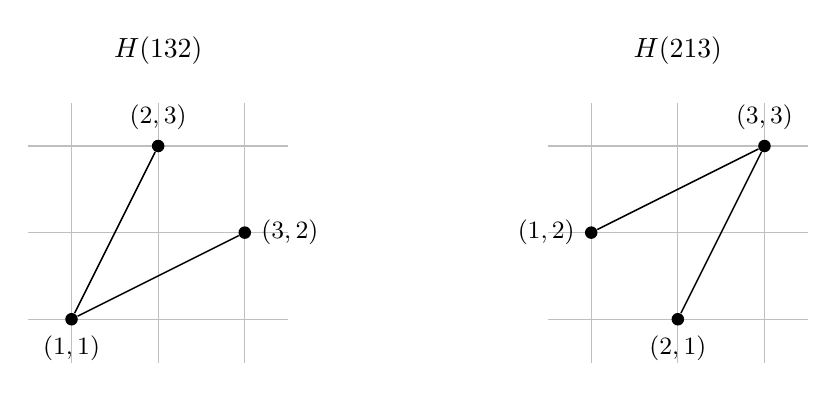
\begin{tikzpicture}[
    scale=1.1,
    vertex/.style={circle, fill=black, inner sep=1.6pt},
    edge/.style={line width=0.55pt},
    gridline/.style={gray!50, thin}
]

% Left: H(132)
\begin{scope}[xshift=0cm]
    \draw[gridline] (0.5,0.5) grid (3.5,3.5);

    \node[vertex,label={[font=\small]below:\((1,1)\)}] (a1) at (1,1) {};
    \node[vertex,label={[font=\small]above:\((2,3)\)}] (a2) at (2,3) {};
    \node[vertex,label={[font=\small]right:\((3,2)\)}] (a3) at (3,2) {};

    \draw[edge] (a1) -- (a2);
    \draw[edge] (a1) -- (a3);

    \node at (2,4.1) {\({H(132)}\)};
\end{scope}

% Right: H(213)
\begin{scope}[xshift=6cm]
    \draw[gridline] (0.5,0.5) grid (3.5,3.5);

    \node[vertex,label={[font=\small]left:\((1,2)\)}] (b1) at (1,2) {};
    \node[vertex,label={[font=\small]below:\((2,1)\)}] (b2) at (2,1) {};
    \node[vertex,label={[font=\small]above:\((3,3)\)}] (b3) at (3,3) {};

    \draw[edge] (b1) -- (b3);
    \draw[edge] (b2) -- (b3);

    \node at (2,4.1) {\({H(213)}\)};
\end{scope}

\end{tikzpicture}
\caption{The induced comparability-grid subgraphs \(H(132)\) and \(H(213)\).}
\end{figure}
\noindent Clearly $H(\pi)$ is isomorphic to $H(\sigma)$ though $\pi \neq \sigma$.
\end{proof}

\begin{fact}
\label{fact:reverse-complement-isomorphic}
Let \(\pi\in S_n\). Define its \term{reverse-complement} by
\begin{align}
    \pi^{\mathrm{rc}}(i)
    &:= n+1-\pi(n+1-i).
\end{align}
Then
$
    H(\pi)\cong H(\pi^{\mathrm{rc}})
$.
\end{fact}

\begin{proof}
Write the vertices of \(H(\pi)\) as
$v_i=(i,\pi(i))$ for $i\in[n]$.
Define
\begin{align}
    f(v_i)
    &:= \bigl(n+1-i,\ n+1-\pi(i)\bigr).
\end{align}
As \(i\) ranges over \([n]\), the image is exactly
\begin{align}
    \{(k,\pi^{\mathrm{rc}}(k)) : k\in[n]\},
\end{align}
so \(f\) is a bijection from \(V(H(\pi))\) to \(V(H(\pi^{\mathrm{rc}}))\).

For \(i\neq j\), adjacency in a comparability grid is given by
\begin{align}
    v_i v_j\in E(H(\pi))
    &\iff (i-j)\bigl(\pi(i)-\pi(j)\bigr)>0.
\end{align}
Under \(f\), both differences change sign:
\begin{align}
    (n+1-i)-(n+1-j)&=-(i-j),\\
    (n+1-\pi(i))-(n+1-\pi(j))
    &= -(\pi(i)-\pi(j)).
\end{align}
Therefore the product
\begin{align}
    (i-j)\bigl(\pi(i)-\pi(j)\bigr)
\end{align}
is preserved. Hence \(v_i v_j\) is an edge if and only if \(f(v_i)f(v_j)\)
is an edge. Thus \(f\) is a graph isomorphism, and $H(\pi)\cong H(\pi^{\mathrm{rc}})$.
\end{proof}

This representation of a subgraph will come very handy in Section \ref{sec:algorihmic-approaches}. We now conclude this section with a few observations regarding whether grids are induced subgraphs of some comparability grid.

\begin{fact}
For all $n \in \N$, $\Grid_{2 \times n}$ is a subgraph of a $\CGrid_{n+1 \times n+1}$.
\end{fact}

\begin{proof}
Repeat and ``untwist'' the following construction: 
\end{proof}
\begin{figure}[H]
\centering
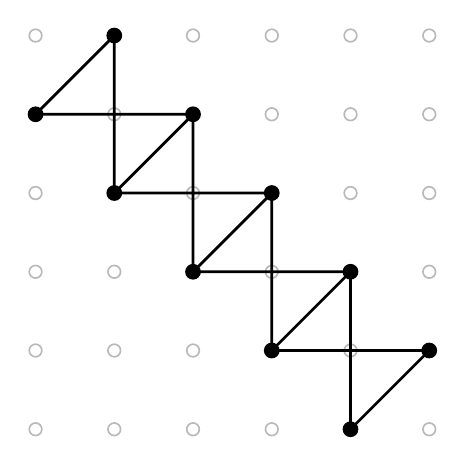
\begin{tikzpicture}[line cap=round, line join=round]

\foreach \x in {0,...,5} {
    \foreach \y in {0,...,5} {
    \draw[gray!55, line width=0.6pt] (\x,\y) circle[radius=0.08];
    }
}

\draw[black, line width=1.0pt]
    (0,4)--(1,5)
    (1,5)--(1,4)
    (0,4)--(1,4)--(2,4)
    (1,4)--(1,3)
    (1,3)--(2,4)
    (1,3)--(2,3)--(2,4)
    (2,3)--(2,2)
    (2,3)--(3,3)
    (2,2)--(3,3)
    (2,2)--(3,2)--(3,3)
    (3,2)--(3,1)
    (3,2)--(4,2)
    (3,1)--(4,2)
    (3,1)--(4,1)--(4,2)
    (4,1)--(4,0)
    (4,1)--(5,1)
    (4,0)--(5,1);

\foreach \p in {(0,4),(1,5),(1,3),(2,4),(2,2),(3,3),(3,1),(4,2),(4,0),(5,1)}{
    \fill[black] \p circle[radius=0.10];
}
\end{tikzpicture}
\caption{A $\Grid_{2 \times 5}$ in a $\CGrid_{6 \times 6}$.}
\label{fig:two-wide-grid-in-cgrid}
\end{figure}

This result is quite exciting, as it immediately implies that $\CGrid$ is 2-qubit universal, as the family of all $\Grid_{2 \times n}$ is 2-qubit universal. Unfortunately, it turns out that we cannot do much better.

\begin{fact}
\label{fact:grid-not-vertex-minor-cgraph}
$\Grid_{3 \times 4}$ is not a vertex minor of any circle graph. Since vertex minors is a strictly more powerful operation than vertex deletion, $\Grid_{3 \times 4}$ is not an induced subgraph of any $\CGrid$.
\end{fact}

\begin{proof}
Look at the following figure:
\begin{figure}[H]
\centering
\begin{tikzpicture}[
    scale=0.8,
    vertex/.style={circle, fill=black, inner sep=1.6pt},
    edge/.style={line width=0.55pt},
    arr/.style={-{Latex[length=2mm]}, line width=0.55pt}
]

% =========================
% Graph 1
% =========================
\begin{scope}[xshift=0cm, yshift=0cm]

\node[vertex] (a11) at (0,3) {};
\node[vertex] (a21) at (1.2,3) {};
\node[vertex] (a31) at (2.4,3) {};

\node[vertex] (a12) at (0,2) {};
\node[vertex] (a22) at (1.2,2) {};
\node[vertex] (a32) at (2.4,2) {};

\node[vertex] (a13) at (0,1) {};
\node (a23) at (1.2,1) {$\times$};
\node[vertex] (a33) at (2.4,1) {};

\node[vertex] (a14) at (0,0) {};
\node[vertex] (a24) at (1.2,0) {};
\node[vertex] (a34) at (2.4,0) {};

\draw[edge] (a11)--(a21)--(a31);
\draw[edge] (a12)--(a22)--(a32);
\draw[edge] (a13)--(a23)--(a33);
\draw[edge] (a14)--(a24)--(a34);

\draw[edge] (a11)--(a12)--(a13)--(a14);
\draw[edge] (a21)--(a22)--(a23)--(a24);
\draw[edge] (a31)--(a32)--(a33)--(a34);

% \node at (1.45,1.02) {\(\star\)};

\end{scope}

\draw[arr] (3.1,1.5) -- (4.2,1.5);

% =========================
% Graph 2
% =========================
\begin{scope}[xshift=4.8cm, yshift=0.05cm]

\node[vertex] (b11) at (0,3) {};
\node[vertex] (b21) at (1.15,3) {};
\node[vertex] (b31) at (2.3,3) {};

\node[vertex] (b12) at (0,2) {};
\node[vertex] (b22) at (1.15,2) {};
\node[vertex] (b32) at (2.3,2) {};

\node[vertex] (b13) at (0,1) {};
\node[vertex] (b33) at (2.3,1) {};

\node[vertex] (b14) at (0,0) {};
\node[vertex] (b24) at (1.15,0) {};
\node[vertex] (b34) at (2.3,0) {};

\draw[edge] (b11)--(b21)--(b31);
\draw[edge] (b12)--(b22)--(b32);
\draw[edge] (b14)--(b24)--(b34);

\draw[edge] (b11)--(b12)--(b13)--(b14);
\draw[edge] (b21)--(b22);
\draw[edge] (b31)--(b32)--(b33)--(b34);

\node at (-0.3,0) {\(\star\)};
\node at (2.6,0) {\(\star\)};

\end{scope}

\draw[arr] (7.75,1.5) -- (8.85,1.5);

% =========================
% Graph 3
% =========================
\begin{scope}[xshift=9.4cm, yshift=0.05cm]

\node[vertex] (b11) at (0,3) {};
\node[vertex] (b21) at (1.15,3) {};
\node[vertex] (b31) at (2.3,3) {};

\node[vertex] (b12) at (0,2) {};
\node[vertex] (b22) at (1.15,2) {};
\node[vertex] (b32) at (2.3,2) {};

\node[vertex] (b13) at (0,1) {};
\node[vertex] (b33) at (2.3,1) {};

\node (b14) at (0,0) {$\times$};
\node[vertex] (b24) at (1.15,0) {};
\node (b34) at (2.3,0) {$\times$};

\draw[edge] (b11)--(b21)--(b31);
\draw[edge] (b12)--(b22)--(b32);
\draw[edge] (b14)--(b24)--(b34);

\draw[edge] (b11)--(b12)--(b13)--(b14);
\draw[edge] (b21)--(b22);
\draw[edge] (b31)--(b32)--(b33)--(b34);

\draw[edge] (b13) -- (b24);
\draw[edge] (b24) -- (b33);

\node at (-0.3,1) {\(\star\)};
\node at (2.6,1) {\(\star\)};

\end{scope}

\draw[arr] (11.9,1.5) -- (13.0,1.5);

% =========================
% Graph 4
% =========================
\begin{scope}[xshift=13.5cm, yshift=0.15cm]

\node[vertex] (b11) at (0,3) {};
\node[vertex] (b21) at (1.15,3) {};
\node[vertex] (b31) at (2.3,3) {};

\node[vertex] (b12) at (0,2) {};
\node[vertex] (b22) at (1.15,2) {};
\node[vertex] (b32) at (2.3,2) {};

\node[] (b13) at (0,1) {$\times$};
\node[] (b33) at (2.3,1) {$\times$};

\node[vertex] (b23) at (1.15,1) {};

\draw[edge] (b11)--(b21)--(b31);
\draw[edge] (b12)--(b22)--(b32);

\draw[edge] (b11)--(b12)--(b13);
\draw[edge] (b21)--(b22);
\draw[edge] (b31)--(b32)--(b33);

\draw[edge] (b13) -- (b23);
\draw[edge] (b23) -- (b33);

\draw[edge] (b12) -- (b23) -- (b32);

% \node at (-0.3,1) {\(\star\)};
% \node at (2.6,1) {\(\star\)};

\end{scope}

\draw[arr] (16.2,1.5) -- (17.3,1.5);

% =========================
% Graph 5
% =========================
\begin{scope}[xshift=17.8cm, yshift=0.2cm]

\node[vertex] (b11) at (0,3) {};
\node[vertex] (b21) at (1.15,3) {};
\node[vertex] (b31) at (2.3,3) {};

\node[vertex] (b12) at (0,2) {};
\node[vertex] (b22) at (1.15,2) {};
\node[vertex] (b32) at (2.3,2) {};

\node[vertex] (b23) at (1.15,1) {};

\draw[edge] (b11)--(b21)--(b31);
\draw[edge] (b12)--(b22)--(b32);

\draw[edge] (b11)--(b12);
\draw[edge] (b21)--(b22);
\draw[edge] (b31)--(b32);

\draw[edge] (b12) -- (b23) -- (b32);

\end{scope}
\end{tikzpicture}
\caption{Vertices marked by \(\star\) are locally complemented, and vertices marked by \(\times\) are deleted. This shows that $\Grid_{3 \times 4}$ has a forbidden minor of circle graphs as a vertex minor.}
\label{fig:grid-has-forbidden-vertex-minor}
\end{figure}
The rightmost graph is a forbidden vertex minor of circle graphs. If the $\Grid_{3 \times 4}$ was the vertex minor of some circle graph, then so would be this forbidden minor. Thus, no circle graph, and consequently no comparability grid, has any $\Grid_{m \times n}$ with $m \geq 3$ and $n \geq 4$ as a vertex minor.
\end{proof}

An exhaustive search (using the algorithms described in the next section) reveals that we may strengthen this result a little bit.

\begin{fact}
\label{fact:grid-3-times-3-not-subgraph}
$\Grid_{3 \times 3}$ is not a induced subgraph of any circle graph. Consequently, $\Grid_{m \times n}$ is not an induced subgraph of any circle graph, for $m,n \geq 3$.
\end{fact}

\begin{proof}
The proof surmounts to enumerating every possible 9-vertex subgraph of a $\CGrid$, and concluding that none are isomorphic to $\Grid_{3 \times 3}$.
\end{proof}

Let us summarize what we have seen this section. Through vertex minors, we see that any potential proof of the universality of the comparability grid cannot involve reducing, via local complementation and vertex deletion, a comparability grid into some desired grid graph. This is the implication of Fact \ref{fact:grid-not-vertex-minor-cgraph}.

Furthermore, if the comparability grid is universal, its MBQC protocol must asymptotically use a strictly super-polynomial or faster growing number of qubits with respect to the number of qubits in the desired output quantum state. This follows from Theorem \ref{thm:cgrid-efficiently-simulable}.

Suppose comparability grids are universal. If we are to present a constructive proof of this, i.e. given a target state $\ket\phi$ on $n$ qubits, an explicit vertex minor of some comparability grid and a measurement pattern that generates $\ket\phi$ using it, then this vertex minor must have asymptotically super-polynomial or larger number of vertices with respect to $n$. In the next section, we outline the key methodology of this thesis: a series of algorithms for enumerating and characterizing the vertex minors of comparability graphs. We run these algorithms to create constructions which we conjecture may show the universality of the comparability grid via a constructive proof. These are presented in Section \ref{sec:conclusions}.